\subsection{Victoria University of Wellington}

Medimos a continuación la ruta a los servidores de la Universidad Victoria en Wellington, Nueva Zelanda. El host de destino elegido fue \emph{'victoria.ac.nz'}.

Realizamos mediciones con 30 iteraciones por TTL y observamos los resultados de la figura \ref{fig:victoria-incrementales}.
\\

\begin{figure}[H]
    \centering
    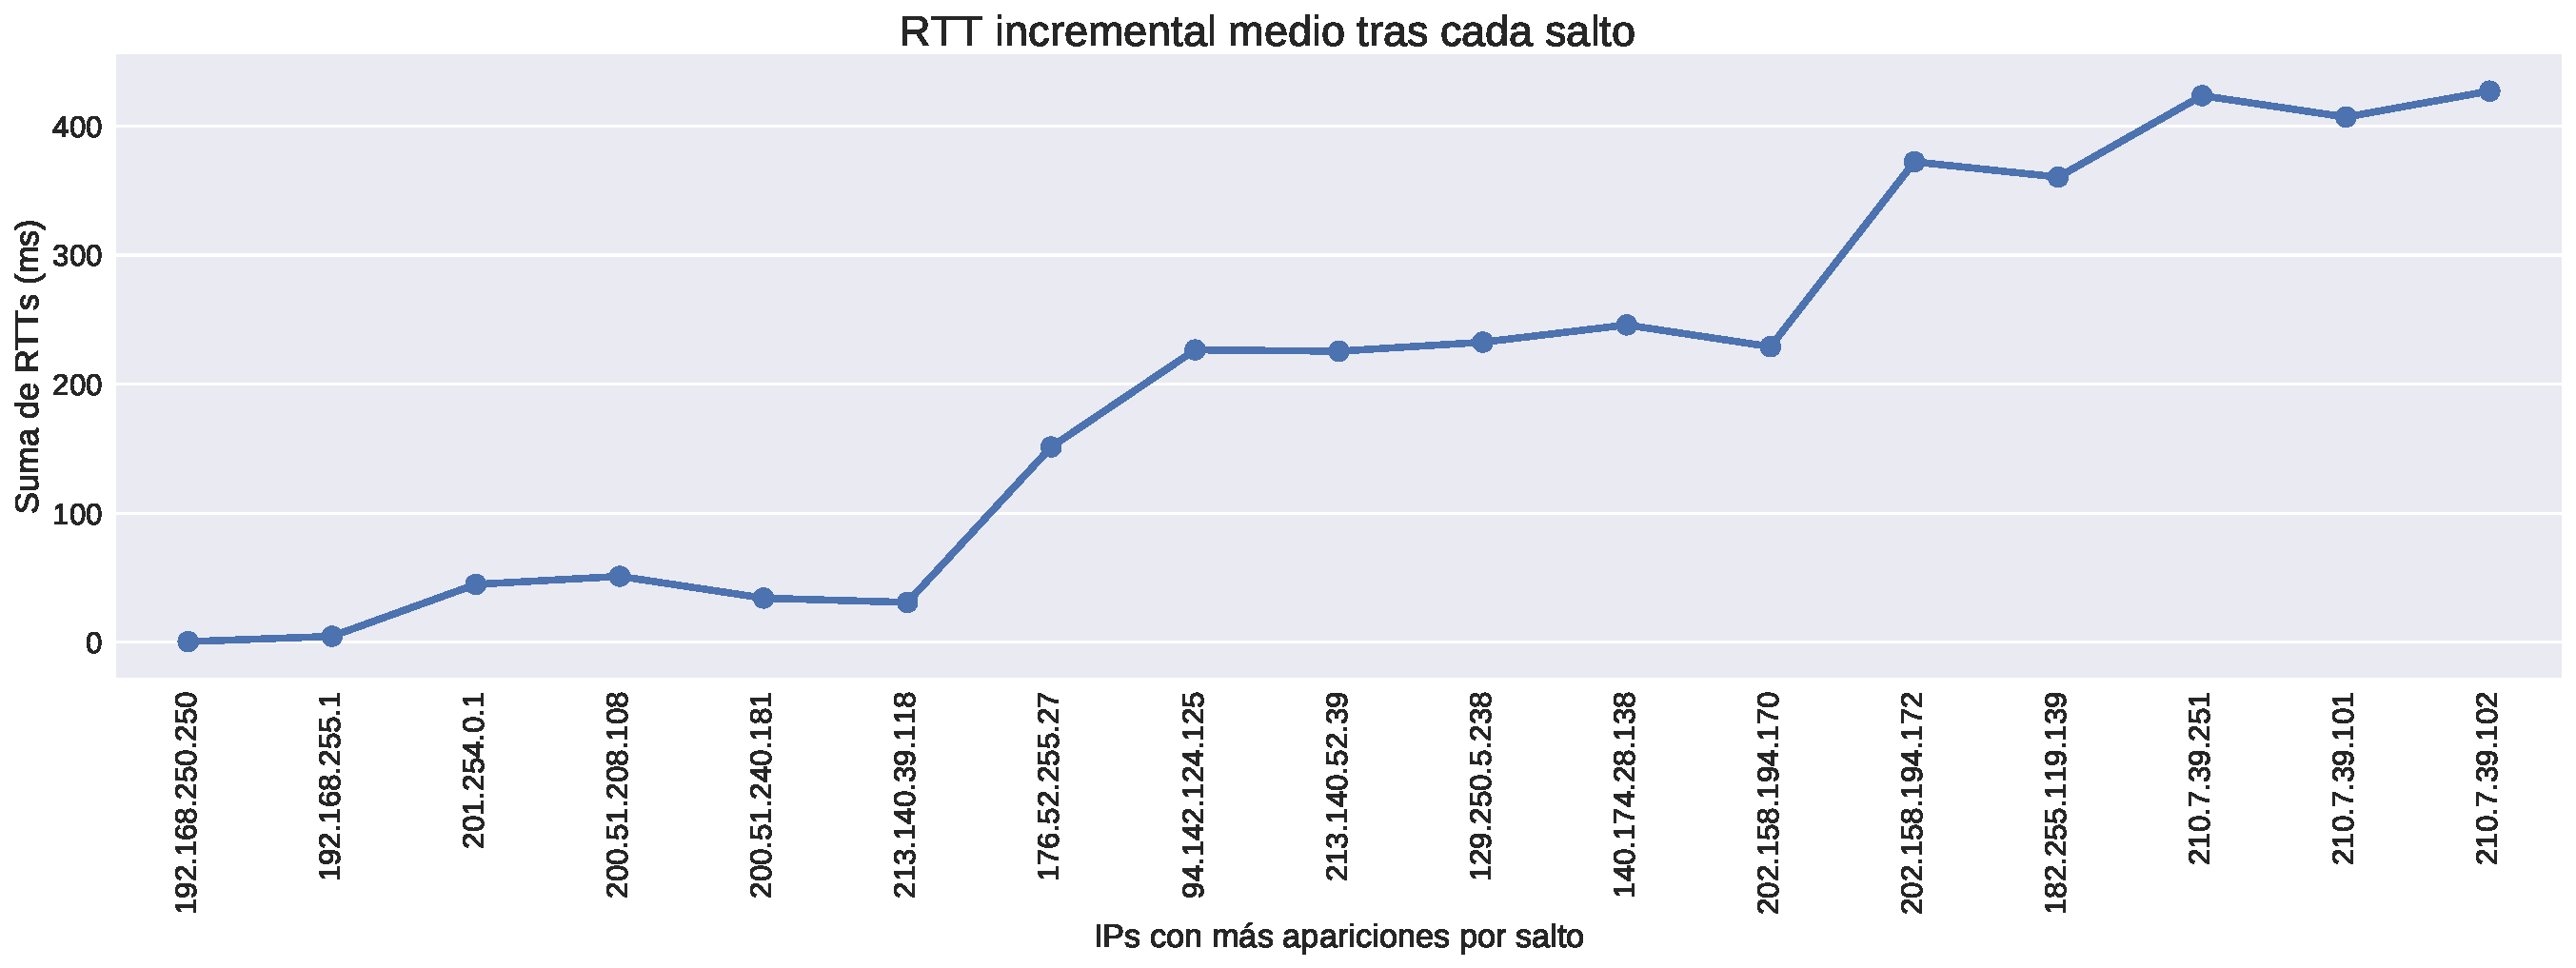
\includegraphics[width=1\textwidth, height=1\textheight, keepaspectratio]{../img/victoria-ac-nz-incrementales}
    \caption{Comportamiento incremental de RTTs medios medidos.}
    \label{fig:victoria-incrementales}
\end{figure}

Notamos tres segmentos distinguidos donde el delay se mantiene relativamente constante.

Hasta la ip $200.51.208.181$ la ruta se encuentra dentro de argentina.
Desde el host $213.140.39.118$ hasta el $213.140.52.39$ nos encontramos con ips que parecen ubicarse en España. Y luego el siguiente host tiene ip estadounidense.
Este comportamiento lo observamos en todas las mediciones realizadas desde la misma red, que utiliza como isp \textit{Speedy}, parte de Telefónica España, por lo que suponemos que los servidores en la ruta de Argentina a Estados Unidos utilizan ips de Telefónica aunque no estén ubicados en España.

Luego de pasar por Estados Unidos nos encontramos con dos ips australianas, $202.158.194.170$ y $202.158.194.172$, entre las cuales se produce el siguiente salto notable.
Debido a la similitud entre ips suponemos que la primera se encuentra realmente en Estados Unidos y se trata de los dos extremos de un cable submarino entre este país y Australia.

Otro salto un poco mas pequeño se produce entre $182.255.119.139$ y $210.7.39.251$ cuando se cambia entre ips australianas y neo zelandesas, por lo que suponemos que se trata de otro cable submarino mas corto.
\\

En la figura \ref{fig:victoria-rtts} se aprecian mas directamente estos tres saltos Argentina - Estados Unidos - Australia - Nueva Zelanda.

\begin{figure}[H]
   \centering
       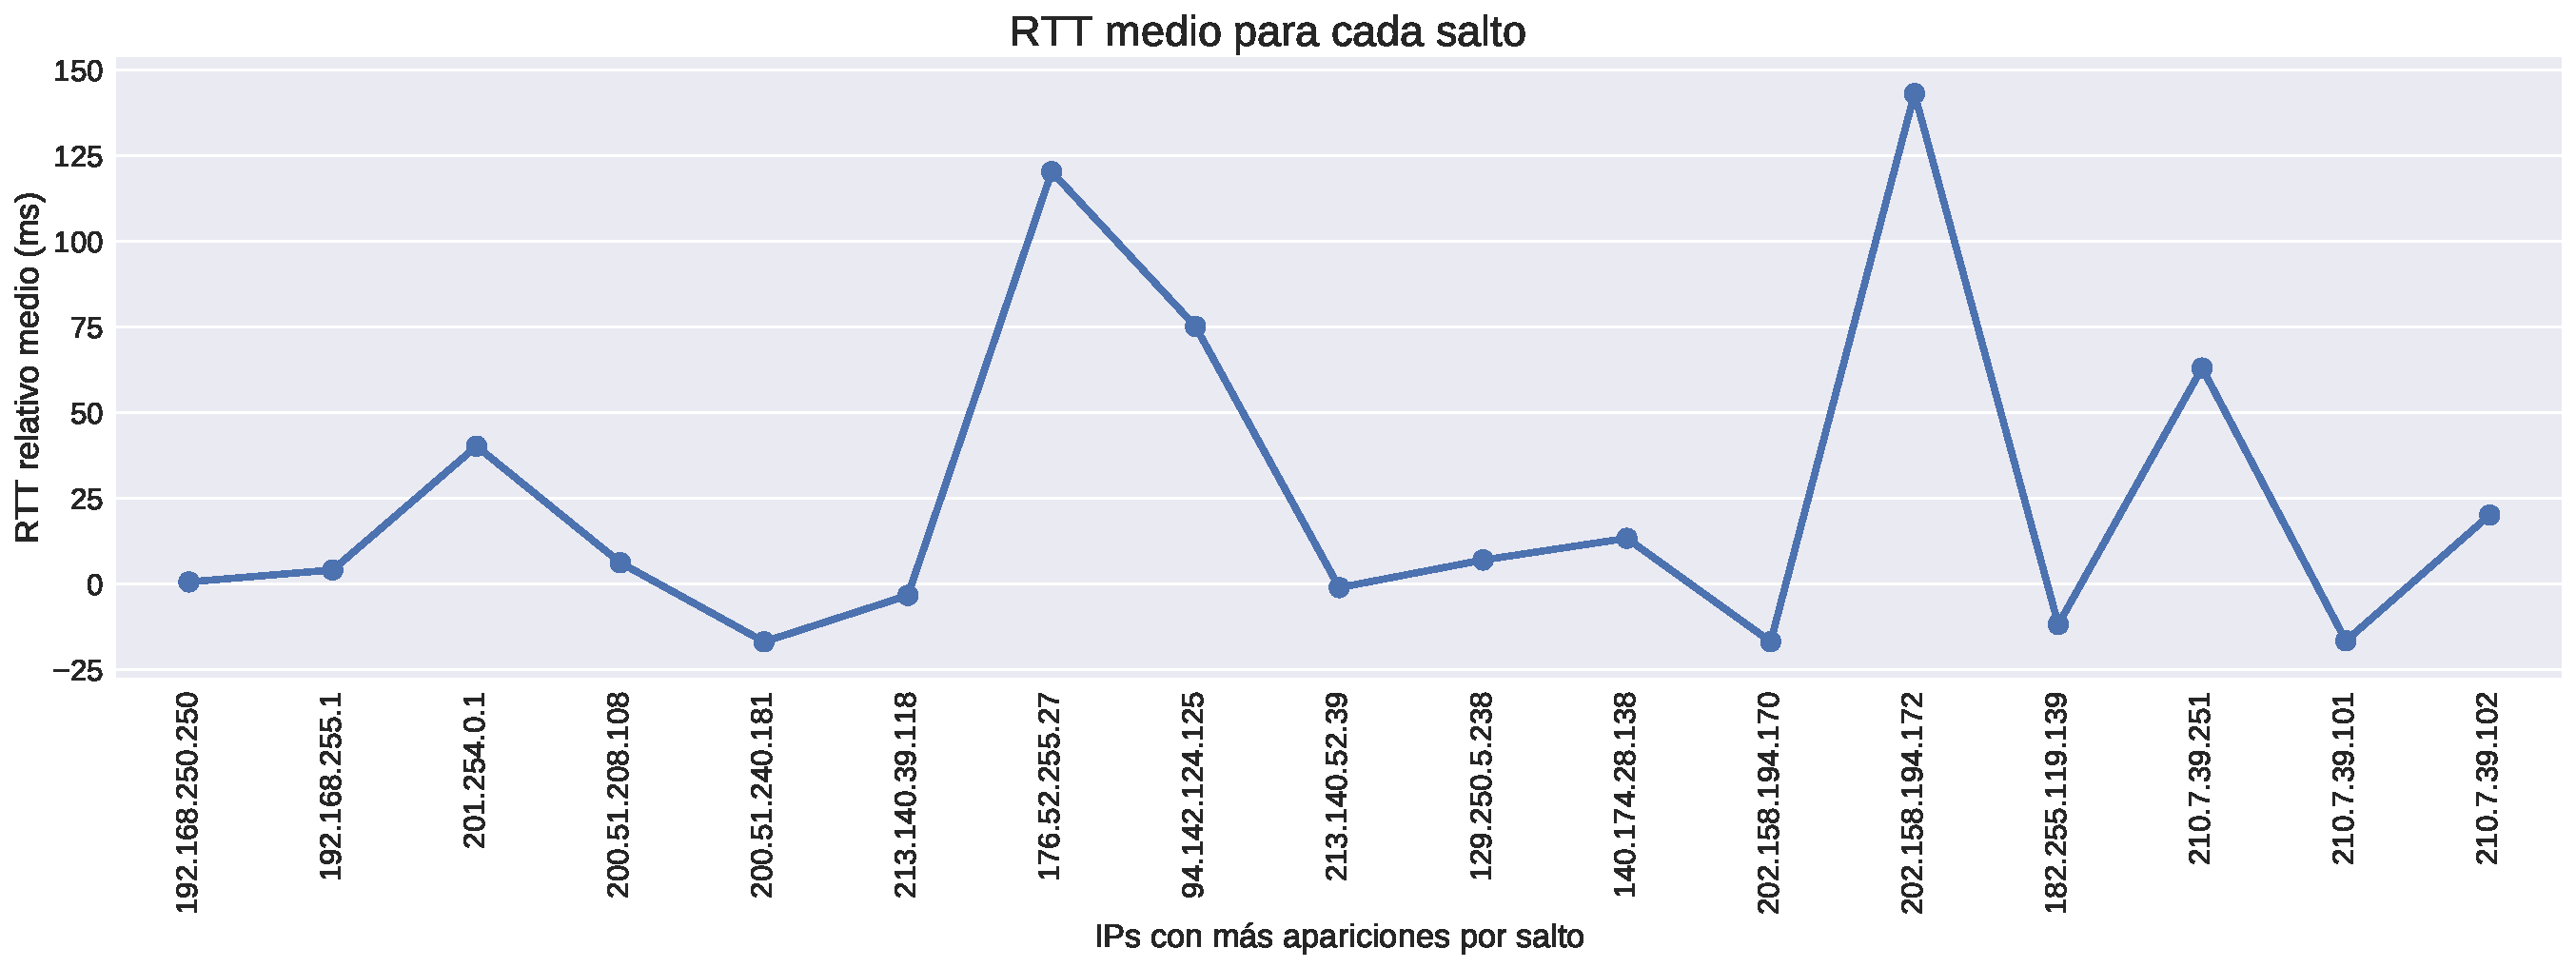
\includegraphics[width=1\textwidth, height=1\textheight, keepaspectratio]{../img/victoria-ac-nz-rtts}
 \caption{RTTs medios medidos para una traceroute a la Universidad Victoria de Wellington.}
 \label{fig:victoria-rtts}
\end{figure}

Vemos en el mapa de la figura \ref{fig:victoria-map} los tramos que nombramos, incluidas las ips españolas, distinguiendo en rojo los que presentaron mayor delay. Debido a que los sectores con mas delay de la ruta se presentaron entre ips del mismo país sólo se marca el cable Australia - Nueva Zelanda.

\begin{figure}[H]
   \centering
       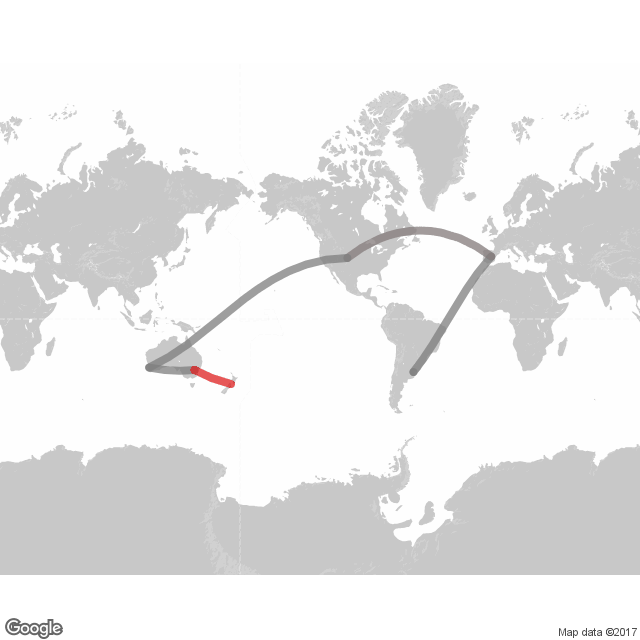
\includegraphics[width=0.5\textwidth, keepaspectratio]{../img/victoria-ac-nz-map}
 \caption{Mapa de ubicaciones inferidas para una traceroute a la Universidad Victoria de Wellington. Tramos con mas delay marcados en rojo.}
 \label{fig:victoria-map}
\end{figure}

En total, 17 de los 19 nodos de la ruta respondieron (un \textbf{89.5}\%).
\\

A continuación intentamos detectar los cables submarinos utilizando el método de Cimbala como se detalló en la sección ~\ref{sec:london}.

Los resultados se pueden apreciar en la figura \ref{fig:victoria-zrtt}. Con el umbral de la tabla $\gamma$ detectamos correctamente el cable entre Argentina y Estados Unidos y entre este y Australia. El tercer cable, de Australia a Nueva Zelanda, no resulta distinguido debido a su poca extensión.

\begin{figure}[H]
   \centering
       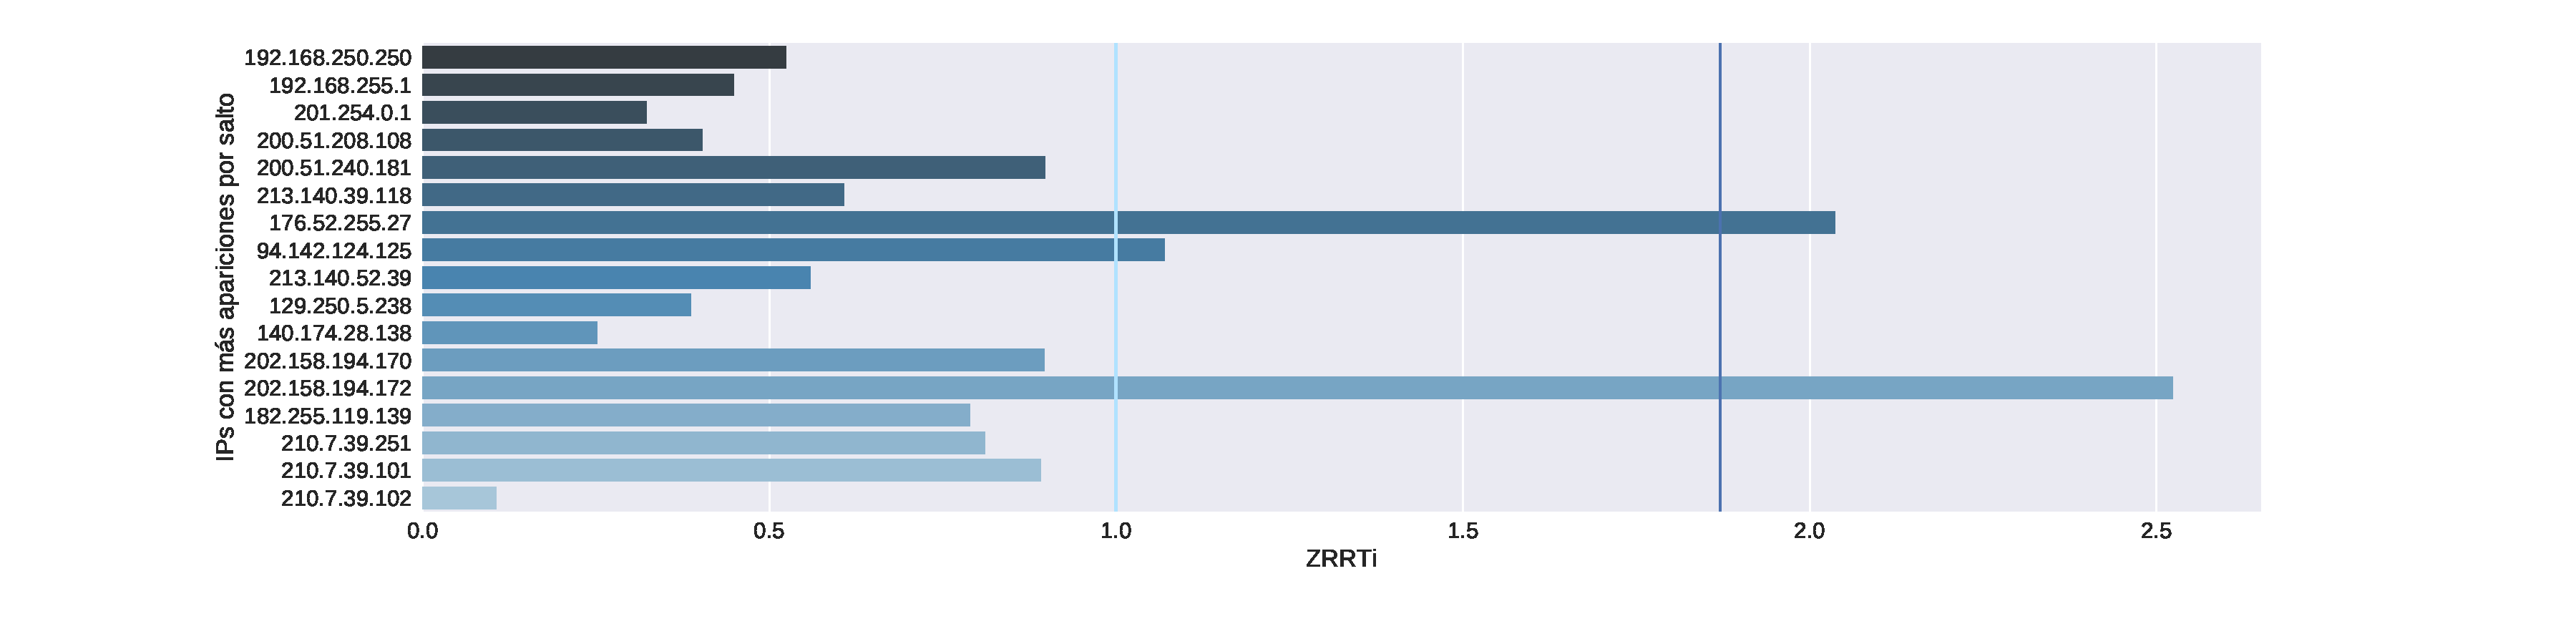
\includegraphics[width=1\textwidth, height=1\textheight, keepaspectratio]{../img/victoria-ac-nz-zrtt}
 \caption{Outliers de la distribución ZRRTi según el método de Cimbala. En azul oscuro: valor $ZRTT_i$ correspondiente a $\tau(n)$ con $n$ el largo de ruta y un alfa fijo (0.05 sugerido en el paper de referencia).}
 \label{fig:victoria-zrtt}
\end{figure}

